\documentclass[a4paper,12pt]{article} % тип документа

\usepackage{tikz}
\usepackage[T2A]{fontenc}			% кодировка
\usepackage[utf8]{inputenc}			% кодировка исходного текста
\usepackage[english,russian]{babel}	% локализация и переносы
\usepackage{amsfonts,longtable}

% Математика
\usepackage{amsmath,amsfonts,amssymb,amsthm,mathtools} 


\usepackage{wasysym}

\title{Лабораторный журнал к работе 1.3.1 по курсу \\ "Общая физика"  \\ 
\vspace{0.2cm}
\vspace{4.5cm}
 \LARGE{\textbf{Определение модуля Юнга на основе исследования деформаций растяженпя и изгиба}}\vspace{5.5cm}}
\date{09.11.2018}
\usepackage{tikz}
\author{\vspace{0.2cm}Баринов Леонид}

\begin{document}
\maketitle
\newpage
\textbf{Цель работы:} Экспериментально получить зависимость между напряжением и деформацией (закон Гука) для двух простейших напряженных состояний упругих тел: одноосного растяжения и чистого изгиба; по результатам измерений вычислить модуль Юнга.

\textbf{В работе используется:} В первой части -- прибор Лермантова, проволка из исследуемого материала, зрительная труба со шкалой, набор грузов, микрометр, рулетка, во второй части -- стойка для изгибания балки, индикатор для измерения величины прогиба, набор исследуемых стержней, грузы, линейка, штангенциркуль.

В первой части работы производим растяжение проволки, и это соответсвует случаю одноосного напряженного состояния, описываемого форумлой 
\[\sigma = E\varepsilon\]
$\sigma$ - напряжение\\
$E$ - модуль Юнга\\
Во второй части работы измерения производят при изгибе балки, которую иногда будем называть бруском, а иногда -- стержнем. Связь между прогибом балки и величиной силы, приложенной посредине между точками опор балки, может быть выражена через модуль Юнга. Это позволяет по измерениям приложенных сил и прогиба определить модуль Юнга.

\section{Определение модуля Юнга по измерениям растяжения проволки}
Для определения модуля Юнга используется прибор Лермантова, схема которого изображена на Рис. 1. Верхний конец проволки П, изготовленной из исследуемого материала, прикреплен к консоли К, а нижний -- к цилиндру, которым оканчивается шарнирный кронштейн Ш. На этот же цилиндр опирается рычаг $r$, связанный с зеркальцем З. Таким образом, удлинение проволоки можно измерить по углу поворота зеркальца.

Натяжение проволоки можно менять, перекладывая грузы с площадки М на площадку О и наоборот. Такая система позволяет исключить влияние деформации кронштейна К на точность изерений, так как нагрузка на нем все время остается постоянной.

При проведении эксперимента следует иметь в виду, что проволока П при отсутствии нагрузки всегда несколько изогнута, что не может не сказываться на результатах, особенно при небольших нагрузках. Проволока вначале не столько растягивается, сколько распрямляется.
\newpage
\begin{figure}[h]
\centering
\includegraphics[scale=0.4]{1}
\caption{Прибор Лермантова}
\end{figure}
\textbf{Ход работы:}
\begin{itemize}
\item Определим площадь поперечного сечения проволки. Для этого измеряем  ее диаметр микрометром не менне чем в десяти местах и во взаимно перпендикулярных напрвлениях в каждом месте. При измерении следим, чтобы микрометр не деформировал проволоку. В дальнейших расчетах надо пользоваться средним значением диаметра, вычисленным по всем измерениям.
\item Измеряем длину проволки
\item Направляем зрительную трубу на зеркальце З. При этом трубу должно быть четко видно отражение шкалы в зеркальце. Выведем формулу, связывающую число делений по шкале $n$, расстояние $h$ от шкалы до зеркальца, длину рычага $r$ и удлинение проволки $\Delta l$
\[\tg\varphi = \frac{\Delta l}{r}\]
$\varphi$ - угол поворота зеркальца
\[\tg 2\varphi = \frac{\Delta n}{n}\]
$\Delta n$ - расстояние между делениями, соответствующие повороту зеркальца на $\varphi$ и начальной нагрузке
В силу малости $\varphi$ $\tg 2\varphi \approx 2 \tg \varphi$
\[2\frac{\Delta l}{r} = \frac{\Delta n}{h}\]
\[\Delta l = \frac{\Delta n r}{2h}\]
Длина рычага указана на приборе, расстояние $h$ измеряем.
\item Позаботимся о том, чтобы в процессе эксперимента не выйти за пределы области, где удлинение проволки пропорционально ее натяжению. Для этого оценим максимальную величину нагрузки, приняв, что разрушающее наряжение равно $900 \frac{H}{\text{мм}^2}$. Рабочее напряжение не должно превышать $30\%$ от разрушающего. Проверим правильность сделанной оценки. Для этого нагрузим проволку одним из имеющихся грузов, затем уберем его и посмотрим, вернулась ли длина проволки к первоначальному значению. Повторим эксперимент с двумя, тремя и т.д. грузами, постепенно доходя до расчетной нагрузки. Если остаточые деформации станут заметными, дальнейшее увеличение нагрузки следует прекратить. При измерении нагрузки на проволоке каждый раз необходимо предварительно арретировать прибор
\item Снимем зависимость удлинения проволоки, то есть числа делений $n$ по шкалы, от массы грузов $m$ при увеличении и уменьшении нагрузки. Повторим эксперимент 2-3 раза.
\end{itemize}
\section{Определение модуля Юнга по измерениям изгиба балки}
Экспериментаьная установка состоит из прочной стойки с опорными призмами А и Б (Рис. 2). На ребра призм опирается исследуемный стержень (балка) В. В середине стержня на призме Д подвешена площадка П с грузами. Измерять стрелу прогиба можно с помощью индикатора И, укрепляемого на отдельной штанге. Полный оборот большой стрелки индикатора соответсвует 1 мм и одному делению малого цифирблата
\newpage
\begin{figure}[h]
\centering
\includegraphics[scale=0.4]{2}
\caption{Схема установки для измерения модуля Юнга}
\end{figure}
Модуль Юнга $E$ материала стержня связан со стрелой прогиба $y_max$ (то есть с перемещением середины стержня) соотношением
\begin{equation}
 E = \frac{P l^3}{4ab^3y_max}
\end{equation}

Здесь $P$ -- нагрузка, вызывающая прогиб стержня, $l$ -расстояние между призмами А и Б, $a$ и $b$ -- ширина и высота сечения стержня.

Чтобы исключить ошибки, возникающие вследствие прогиба стола при изменении нагрузки на стержень, грузы перед началом эксперимента следует расположить на рейке над нижней полкой опорной стоки.

Формула (1) была выведена при условиях, что, во-первых, ребра опорных призм А и Б находятся на одной горизонтали (высоте) и, во-вторых, сила $P$ приложена точно посередине балки.

\textbf{Ход работы:}
\begin{itemize}
\item Измеряем расстояние между ребрами призм А и Б.
\item Определяем ширину и толщину балки (стержня). Для этого измеряем указанные параметры не менее чем в десяти различных местах. По ним вычисляем средние значения, которые будут использованы в дальнейших расчетах.
\item Исследуемую балку положим на стойку. Установим индикатор в центре балки и снимим зависимость стрелы прогиба $y_max$ от велечины нагрузки $P$. Измерения проделаем при возростании и убывании нагрузки. Проверим, возвращается ли балка в первоначальное положение после снятия нагрузки. 
\item Исследуем, насколько существенна зависимость результата от положения точки приложения изгибающей силы $P$ Для этого сместим призму Д на 2-3 мм от точки, принятой за середину балки, и вновь измерим стрелу прогиба. Эту величину сравним с результатом, полученным при положении призмы Д посередине балки.
\item Перевернем балку таким образом, чтобы при нагружении она изгибалась в противоположную сторону, и повторим измерения. Сравним результаты с предыдущими.
\item Аналогичные измерения измерения проведем для 2-3 баллок, изготовленных из дерева, и одной металлической.
\end{itemize}
\section{Обработка данных}
\end{document}